% !TEX root = ../main.tex


\section{Results}
The first sound clip we tried to alter with the chorus effect, was the strumming of a chord on the guitar. This sound clip was specific selected because the chorus effect should be prominent on string instruments. 
In \colorbox{red}{figure...},the result of the chorus effect in the time domain is shown. Since the delay is only \SI{30}{\milli\second} it is difficult to see any effect on the visualized data. Meanwhile by listening to the signal in audio format revivals a big difference. This is to be expected thus the small delays introduced by the chorus modulation gives rise to tiny frequency changes. These tiny varying frequency changes leads to a so call beat frequency effect which are easily detected by the ear.

With such small changes in frequency a more scattered frequency spectrum ought to be expected, which is also the case as shown in \colorbox{red}{figure}. The scattering occurs when the frequency bins is not small enough to cover all the present frequencies.
   
\fxnote{indsæt billede af tidsdomæne guitar}
\fxnote{indsæt billede af frekvensdomæne}




%In the chorus effect, when you compare the 2 sound clips the one before the chorus affect is added and the one after.
%You notice a more smoothness of tone and the sound of extra trumpets especially jumps out at you which really gives the appearance of grandeur.
%the difference can also be seen visually by inspecting figure \ref{fig:monkeyIslandchorus} and \ref{fig:monkeyIsland} which shows the signal before and after chorus effect was added.

%\begin{figure}[!hbt]
%	\centering
%	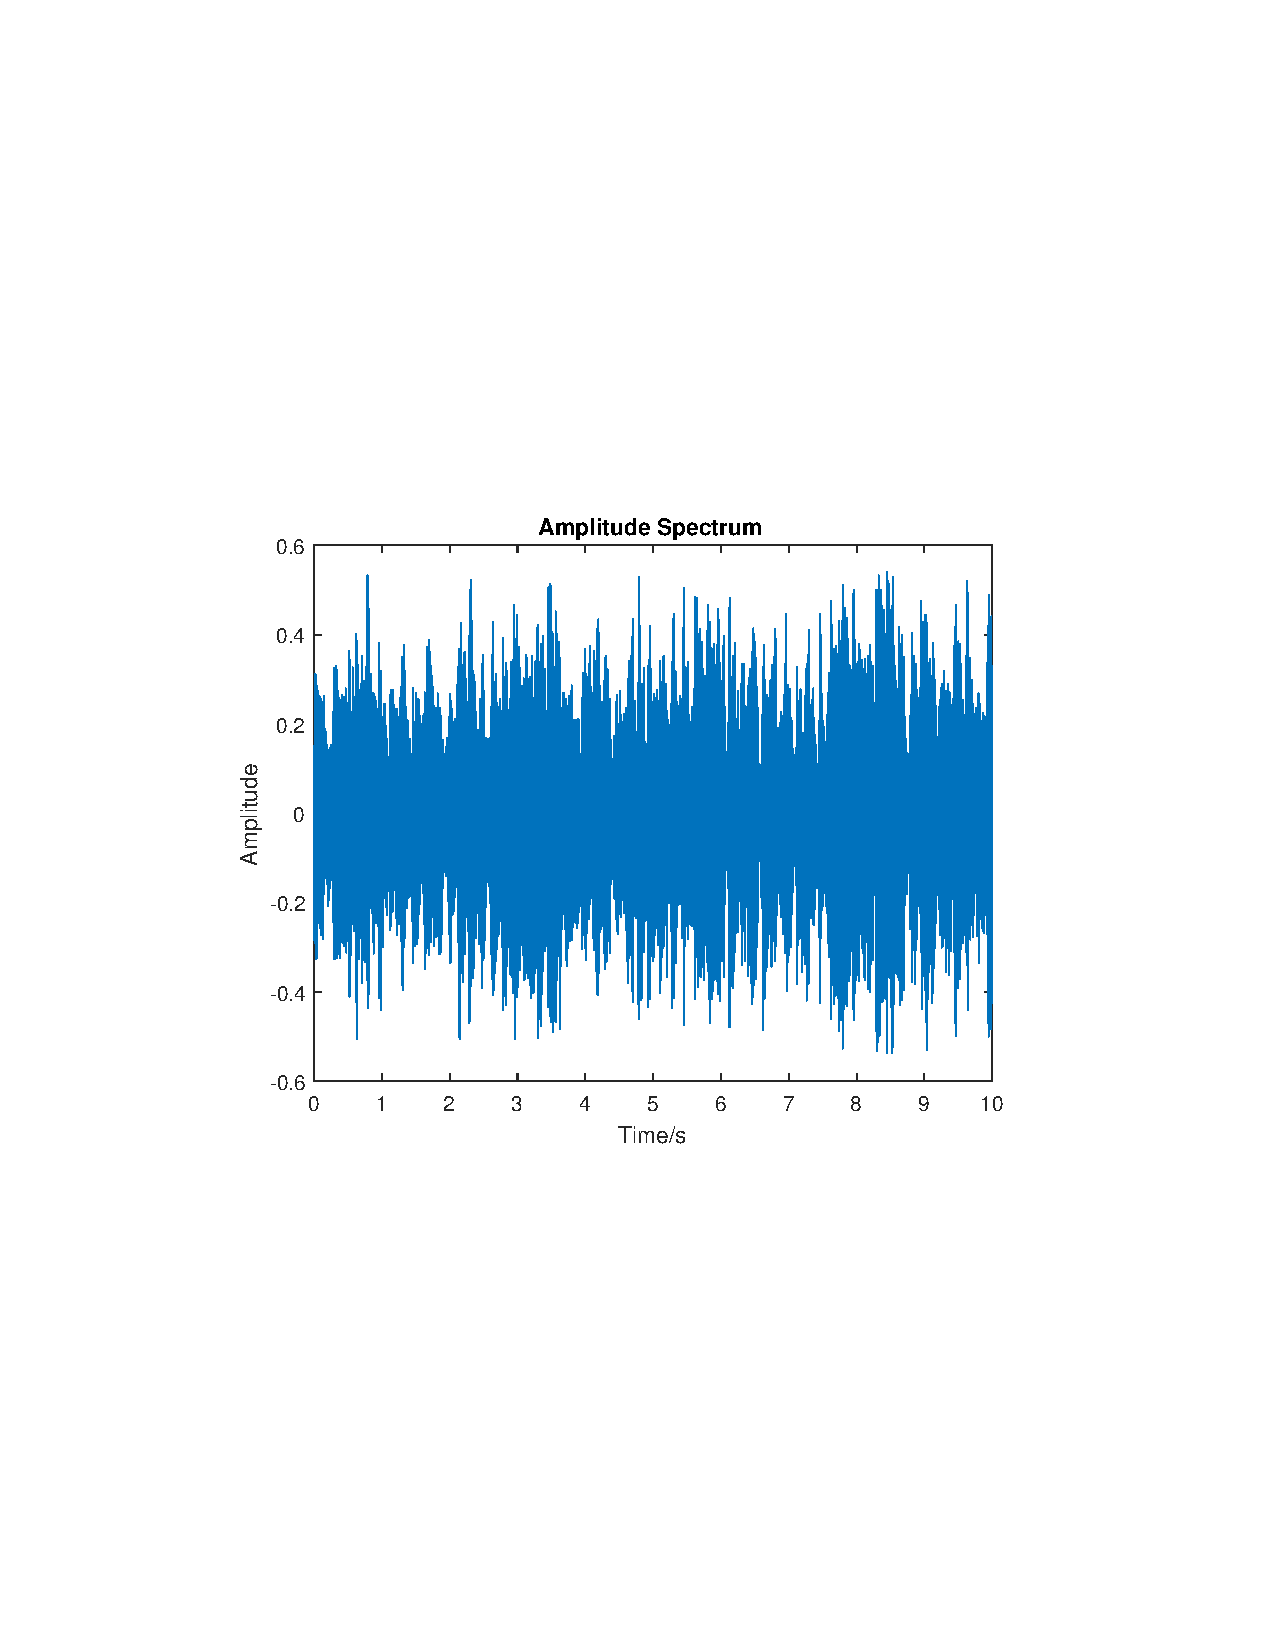
\includegraphics[width=\textwidth]{monkeyIslandchorus.pdf}
%	\caption{Excerpt of the theme from Monkey Island in the time domain, with the chorus effect added .}
%	\label{fig:monkeyIslandchorus}
%\end{figure}

